%%TODO: Label setzen\

%Dokument erstellen
\documentclass[a4paper,DIV11,bibliography=totoc,headings=normal,ngerman,headsepline,listof=totoc,parskip=half]{scrreprt}

%Benötigte Packages
\usepackage{babel} 
\usepackage[T1]{fontenc}           
\usepackage[utf8]{inputenc}  
\usepackage{graphicx}
\usepackage{amsmath}
\usepackage{lmodern}

%Literaturverzeichnis
%\usepackage[babel,german=quotes]{csquotes}
%\usepackage[backend=biber]{biblatex}
\bibliographystyle{plain}

%Formelverzeichnis mittels KOMA-Script erstellen
\DeclareNewTOC[type=formel,name={Formel},hang=5em,listname={Formelverzeichnis}]{for}
\newcommand*{\formelentry}[1]{\addcontentsline{for}{formel}{\protect\numberline{Formel~\theequation} #1}}

%Informationen der PDF
\pdfinfo
{
/Title		(Extrapolation von Zeitreihen mit Hilfe von künstlichen neuronalen Netzen am Beispiel von Börsenprognosen)
/Subject	(Eine Anwendung im Fach Softcomputing – Teilgebiet neuronale Netze)
/Author		(Sebastian Schötteler \& Benedikt Hofrichter)
}

%Kopf- und Fußzeile
\pagestyle{headings}

\begin{document}

\subject{Seminararbeit}
\title{Extrapolation von Zeitreihen mit Hilfe von künstlichen neuronalen Netzen am Beispiel von Börsenprognosen}
\author{Sebastian Schötteler -- Matrikelnummer 2429289 \and Benedikt Hofrichter -- Matrikelnummer 2272198}
\subtitle{\bigskip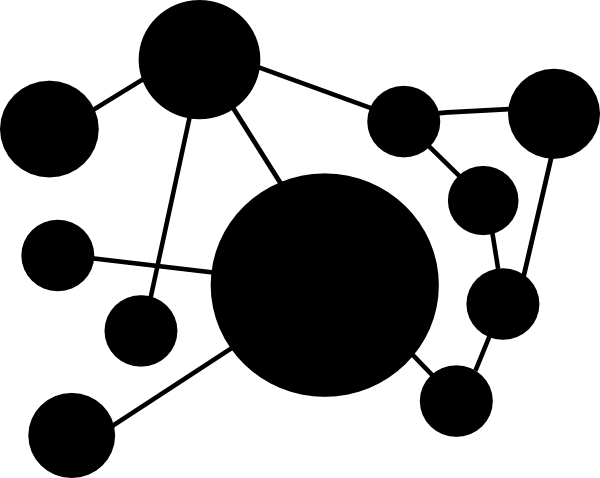
\includegraphics[width=50mm]{titelbild.png}} 
\publishers{
\includegraphics[width=100mm]{TH-Logo.jpg}}

%Zur Überscchrift machen
\maketitle

\pagenumbering{Roman}
%Verzeichnisse
\tableofcontents
\listoffigures
\listoftables
\listofformels

%Text startet hier
\chapter{Einleitung} %Beide
 \pagenumbering{arabic}
\label{cha:Einleitung}
\section{Motivation}
\label{sec:Motivation}
Die Untersuchung und Extrapolation von Zeitreihen ist ein bedeutendes Thema in zahlreichen Gebieten. Typische Anwendungsbereiche sind zum Beispiel die Prognose von Wetterdaten, von Therapieverläufen in der  Medizin, von Arbeitslosenzahlen auf dem Arbeitsmarkt sowie von Börsenkursen. Um eine Zeitreihe möglichst genau zu extrapolieren, wird auf mehreren Hilfsmitteln zurückgegriffen. Einer dieser Hilfsmittel können künstliche neuronale Netze sein. 

Bei künstlichen neuronalen Netzen handelt es sich um Netzwerke mit künstlichen Neuronen als Knoten, die mittels gerichtete Verbindungen Eingaben einlesen, weiterverarbeiten und die daraus resultierenden Ergebnisse an weitere Neuronen weiterleiten oder als Ergebnis ausgeben. Bei der Terminologie von künstlichen neuronalen Netzen wird bewusst auf Begriffen der Biologie zurückgegriffen, da künstliche neuronale Netze das biologische Gehirn als Vorbild nutzen und dessen Herangehensweise auf analoger Weise umzusetzen zu versuchen. Man nennt das Verfahren dieser Netze aus diesem Grunde auch \textit{naturanaloge Verfahren}.

Warum sind diese Netze nun so interessant für Prognosen? Das Erstellen von zum Beispiel Börsenprognosen basiert in der Regel auf Auswertungen von Informationen verschiedenster Quellen. Die Art von Auswertungen, wie Börsenexperten sie vornehmen, ist weder vollständig formalisierbar noch besonders exakt, da uneinheitlich und in weiten Zügen intuitiv. Besonders schwer ist hier das Ermitteln von \textit{nichtlinearen Zusammenhängen}. Ein künstliches neuronales Netz ist jedoch in der Lage, diese Zusammenhänge zu finden  und diese objektiv und vorurteilsfrei zu bewerten. Somit sind künstliche neuronale Netze prinzipiell in der Lage, jedes beliebige Muster in jedem beliebigen Markt zu erkennen - auch solche, die noch nie zuvor von irgend jemand entdeckt wurden.

Ob und wie gut künstliche neuronale Netze zur Prognose geeignet sind, ist pauschal nicht zu beantworten. In manchen Gebieten mag die Prognosefähigkeit durchaus ausreichen. Je höher die geforderte Genauigkeit jedoch wird, desto diskutabler wird ein Einsatz von künstlichen neuronalen Netzen. Eine typische Grauzone ist hier die Prognose von Börsenkursen. Während Befürworter auf die Eigenschaft von künstlichen neuronalen Netzen hinweisen, nichtlineare Muster zu erkennen und entsprechend zu behandeln, argumentieren Kritiker, dass ein System, das dem menschlichen Lernen nachempfunden wurde die gleichen Fehler machen wird wie der Mensch. Generell ist jedoch zu sagen, das die Prognosequalität von künstlichen neuronalen Netzen stets angestiegen ist.


\section{Ziel und Aufbau dieser Arbeit}
\label{sec:Ziel}
Die Funktionsweise und Effektivität von KNN bei der Extrapolation von Zeitreihen soll anhand einer Anwendung, die den Börsenkurs des DAX für die nächsten Börsentage prognostiziert, ermittelt und anschließend demonstriert werden.
\ref{cha:Einleitung}
 
\chapter{Konzeption} %Beide
\label{cha:Konzeption}
\section{Fachliche Konzeption der Anwendung} %Benedikt
\label{sec:Konzeption Anwendung}

\begin{figure}[htbp]3
\centering
		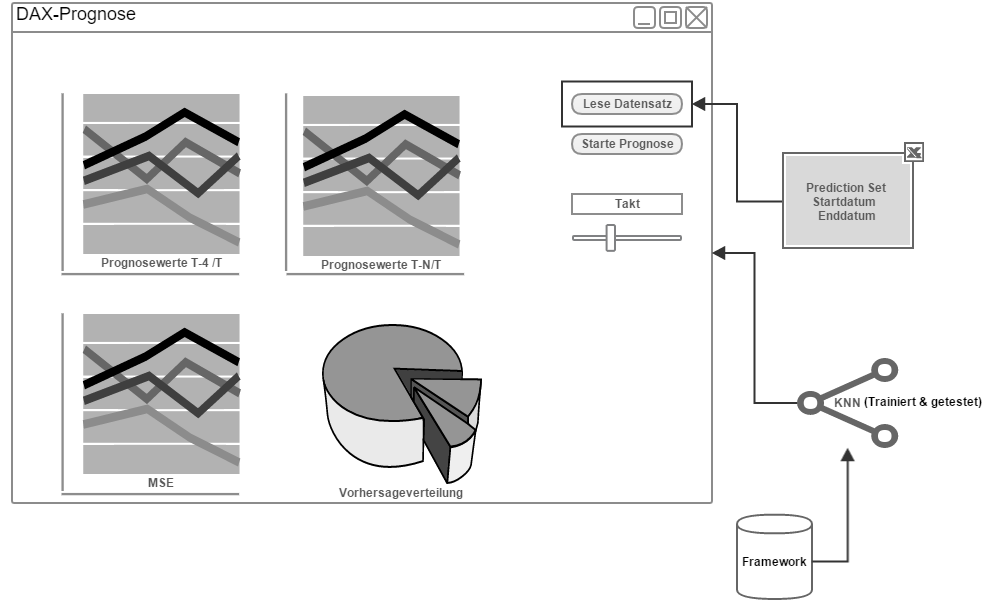
\includegraphics[width=0.80\textwidth]{mockup.PNG}
	\caption{Mockup der Anwendung}
	\label{fig:Mockup der Anwendung}
\end{figure}


\section{Konzeption des künstlichen neuronalen Netzes} %Sebastian
\subsection{Typ des künstlichen neuronalen Netzes} %Sebastian
\subsection{Architektur des künstlichen neuronalen Netzes} %Sebastian
\subsection{Lernverfahren des künstlichen neuronalen Netzes} %Sebastian
\section{Beschreibung von Frameworks} %Benedikt
\subsection{SNNS} %Benedikt
\subsection{JavaNNS}  %Benedikt
\subsection{Neuroph} %Benedikt
\section{Wahl des geeignetsten Frameworks} %Benedikt
\chapter{Umsetzung} %Beide
\section{Erstellung des künstlichen neuronalen Netzes} %Sebastian

\subsection{Wahl der Topologie} %Sebastian
In der Literatur wird dabei oft auf die folgende Gleichung zur Ermittlung der optimalen  Menge an Neuronen der versteckten Schicht angegeben:

\begin{equation}\formelentry{Optimale Anzahl Neuronen in der versteckten Schicht}
  N_h = \frac{N_d}{10*(N_i+N_o)}
\end{equation}

\subsection{Wahl der Transferfunktion} %Sebastian

Sigmoide Funktion:

\begin{equation}\formelentry{Sigmoide Funktion}
f(x)= \frac{1}{1+e^{-cx}}
\end{equation}

Tangens Hyperbolicus:

\begin{equation}\formelentry{Tanh Funktion}
f(x)= tanh(x)
\end{equation}

\subsection{Wahl der Lernregel} %Sebastian
\section{Überführung des künstlichen neuronalen Netzes in einer Anwendung}
\section{Umsetzen der Anwendung} %Benedikt

\chapter{Beschreibung der Anwendung} %Benedikt
\section{Elemente der GUI} %Beide
\section{Architektur der Anwendung} %Benedikt

\chapter{Fazit} %Beide
\label{cha:Fazit}
Das prognostizieren von Börsenkursen mittels künstlichen neuronalen Netzen ist möglich.

%Literaturverzeichnis anzeigen
\bibliography{Literatur}

\end{document}